This section will introduce and develop the \rrtfunnel{} algorithm, by two
means: First develop robust motion primitives through the \ac{SOS} programming
framework based on the work by \cite{majumdarFunnelLibrariesRealtime2017},
and second, deploy these funnels as robust motion primitives in a discrete
\ac{RRT} robust motion planner based on \cite{Lav06}. Using robust motion
primitives has several advantages. Firstly, they handle uncertainty, and thus,
as long as the uncertainties in the system are akin to the assumptions on the
incoming uncertainty parameters, the dynamical system will not leave the funnel,
and hence if the funnel is not in collision, neither will the system be.
Secondly, as the motion primitives are robust, there is no need for more
conservative maneuvers and heuristics, such as maximizing the distance to an
obstacle, which many motion planners do in order to handle uncertainty. Since
the primitives are robust, the system might as well choose a primitive that is
close to an obstacle, as one that is far away, since the funnel is guaranteed to
be collision-free in both cases. This means that a robust motion algorithm can
perform more aggressive maneuvers than one that is inherently conservative about
its environment and maneuvers~\cite{singhRobustOnlineMotion2017}.


\subsection{Generating Robust Motion Primitives}
\label{sec:generating-robust-motion-primitives}

In order to create a basic set of funnels as the robust motion primitives for
the \rrtfunnel{} motion planning algorithm, a few obstacles has to be overcome.
The first one is settling on a dynamical system model for the funnel
calculations. This thesis employs the simple unicycle model from
\author{Lav06}~\cite[613]{Lav06} which is modified slightly into
\begin{equation}
  \label{eq:model-dynamics}
  \vect{x} =
  \begin{bmatrix}
    x \\ y \\ \theta \\
  \end{bmatrix}, \, \dot{\vect{x}} =
  \begin{bmatrix}
    -v \sin(\theta) \\
    v \cos(\theta) \\
    u \\
  \end{bmatrix}
  ,
\end{equation}
which is a first-order unicycle model with constant speed of
\(v=10\) \IEEEunit{m/s}. A picture of the model can be found in
\cref{fig:second-order-unicycle}.
\begin{figure}[!t]
  \def\svgwidth{\columnwidth}
  \import{figures/method/}{unicycle-model.pdf_tex}
  \caption{The unicycle model of an airplane.}
  \label{fig:second-order-unicycle}
\end{figure}
Although this is the only model used in this thesis, the framework and the code
is easily adapted into accommodating a different and more complicated model.


\subsubsection{Generating Trajectories}
\label{subsec:generating-the-trajectories}

The robust motion primitives are \textit{finite regions of time variance} around
an initial trajectory, meaning that they are all the states surrounding a
trajectory in which the system can reach in a given time. But in order to verify
the robust regions surrounding a trajectory, first the trajectories themselves
have to be generated. Generating optimal trajectories is a rich field in the
motion planning literature~\cite{Betts_1998}. The initial trajectories can be
generated by many different methods, however the \textit{direct collocation
  method} suited the needs of this thesis best~\cite{von1993numerical}. It was
chosen as it builds locally optimal trajectories from a discrete set of sampled
points along a sought trajectory, which is beneficial for the discrete funnel
verification in \cref{subsec:generating-funnels}. All optimal trajectory
generators need a cost function to optimize. For this problem the cost function
chosen for the solver to minimize is:
\begin{equation}
  J = \int_{0}^{T} \left[ 1 + {\vect{u}_{0}}^{T} \matr{R} \vect{u}_{0} \right] \mathrm{d}t,
\end{equation}
where \(\matr{R} = 1\), because it will minimize the system input, and thus give
a smooth output trajectory~\cite{majumdarRobustOnlineMotion2013}.

An example of an initial trajectory set generated with the direct collocation
method, and the given cost function is pictured
in~\cref{fig:initial-trajectories}, and consists of a left-turn, a
straight-forward, and a right-turn trajector.

\begin{figure}[!t]
  \begin{minipage}[t]{0.3\linewidth}
    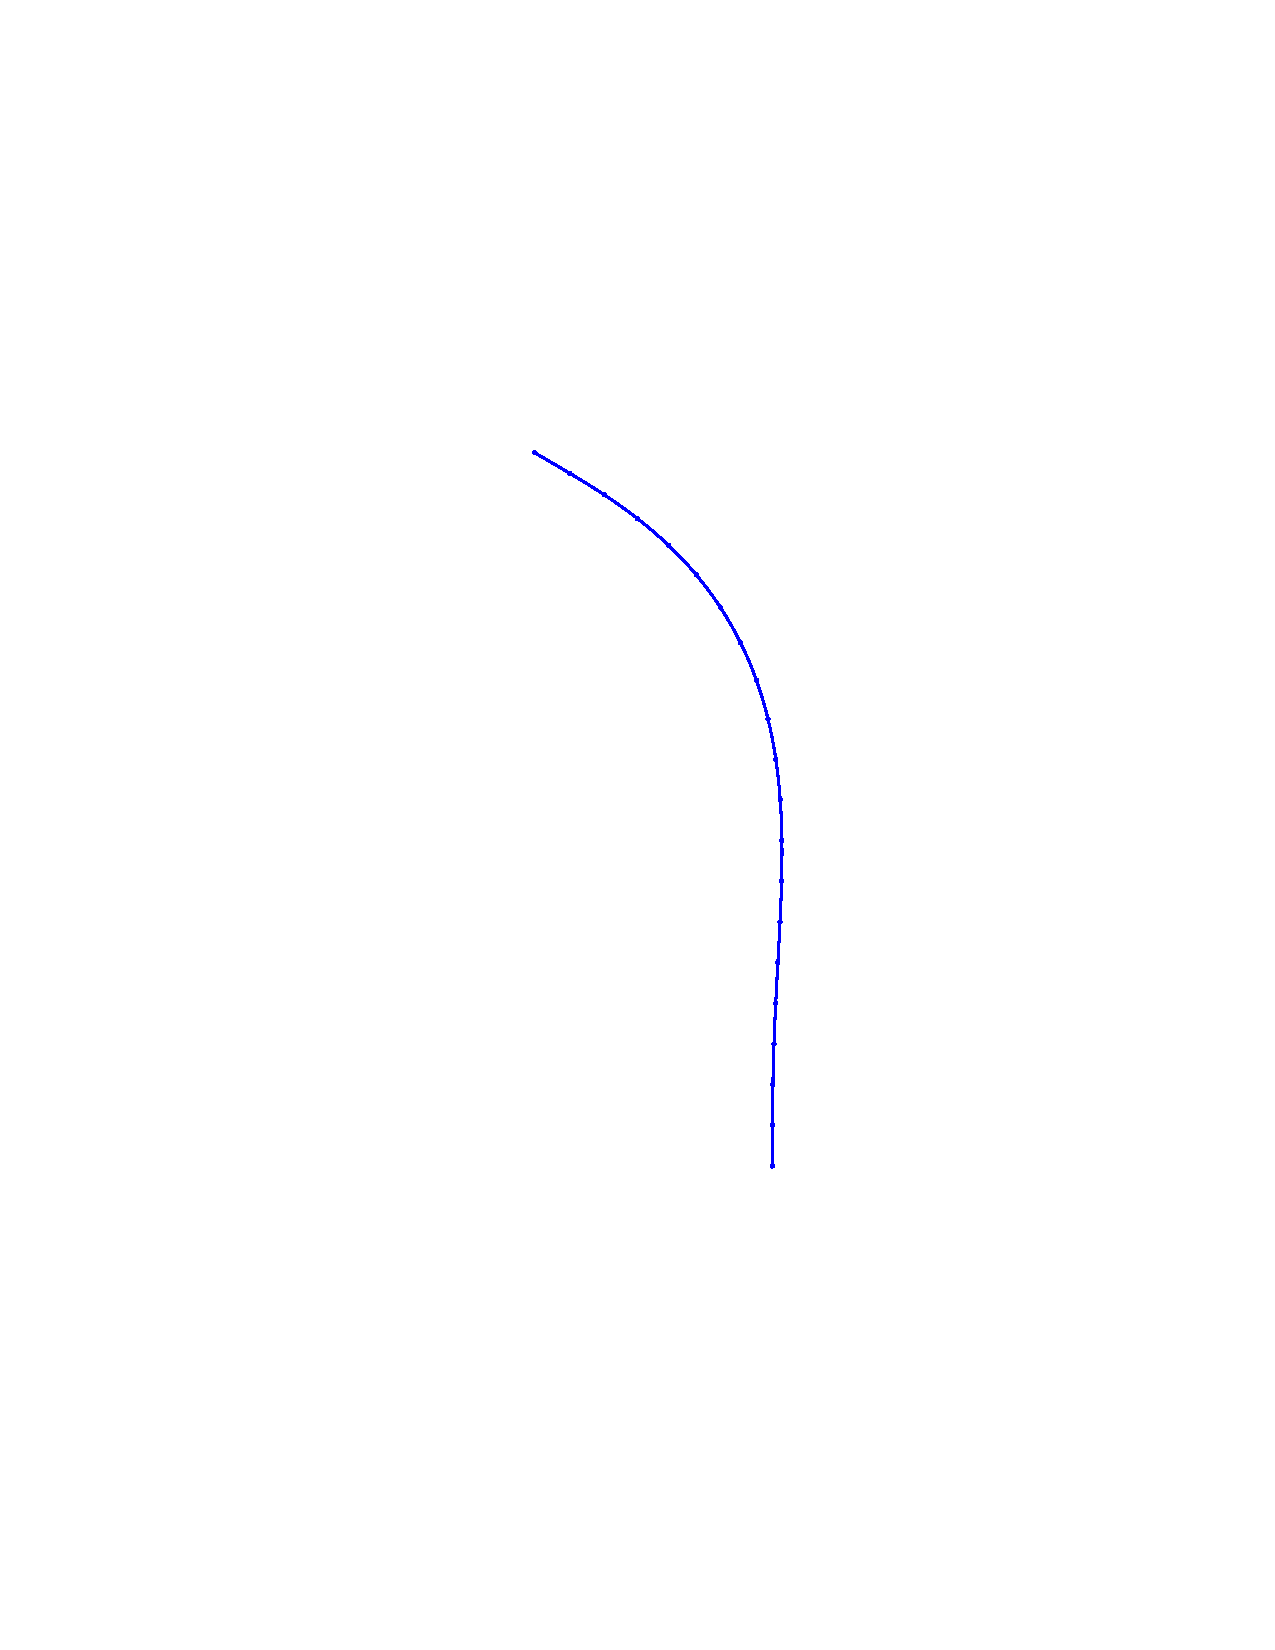
\includegraphics[trim={5cm 5cm 5cm 5cm},
    width=.85\linewidth]{figures/method/left-trajector}
  \end{minipage}
  \hfill
  \begin{minipage}[t]{0.3\linewidth}
    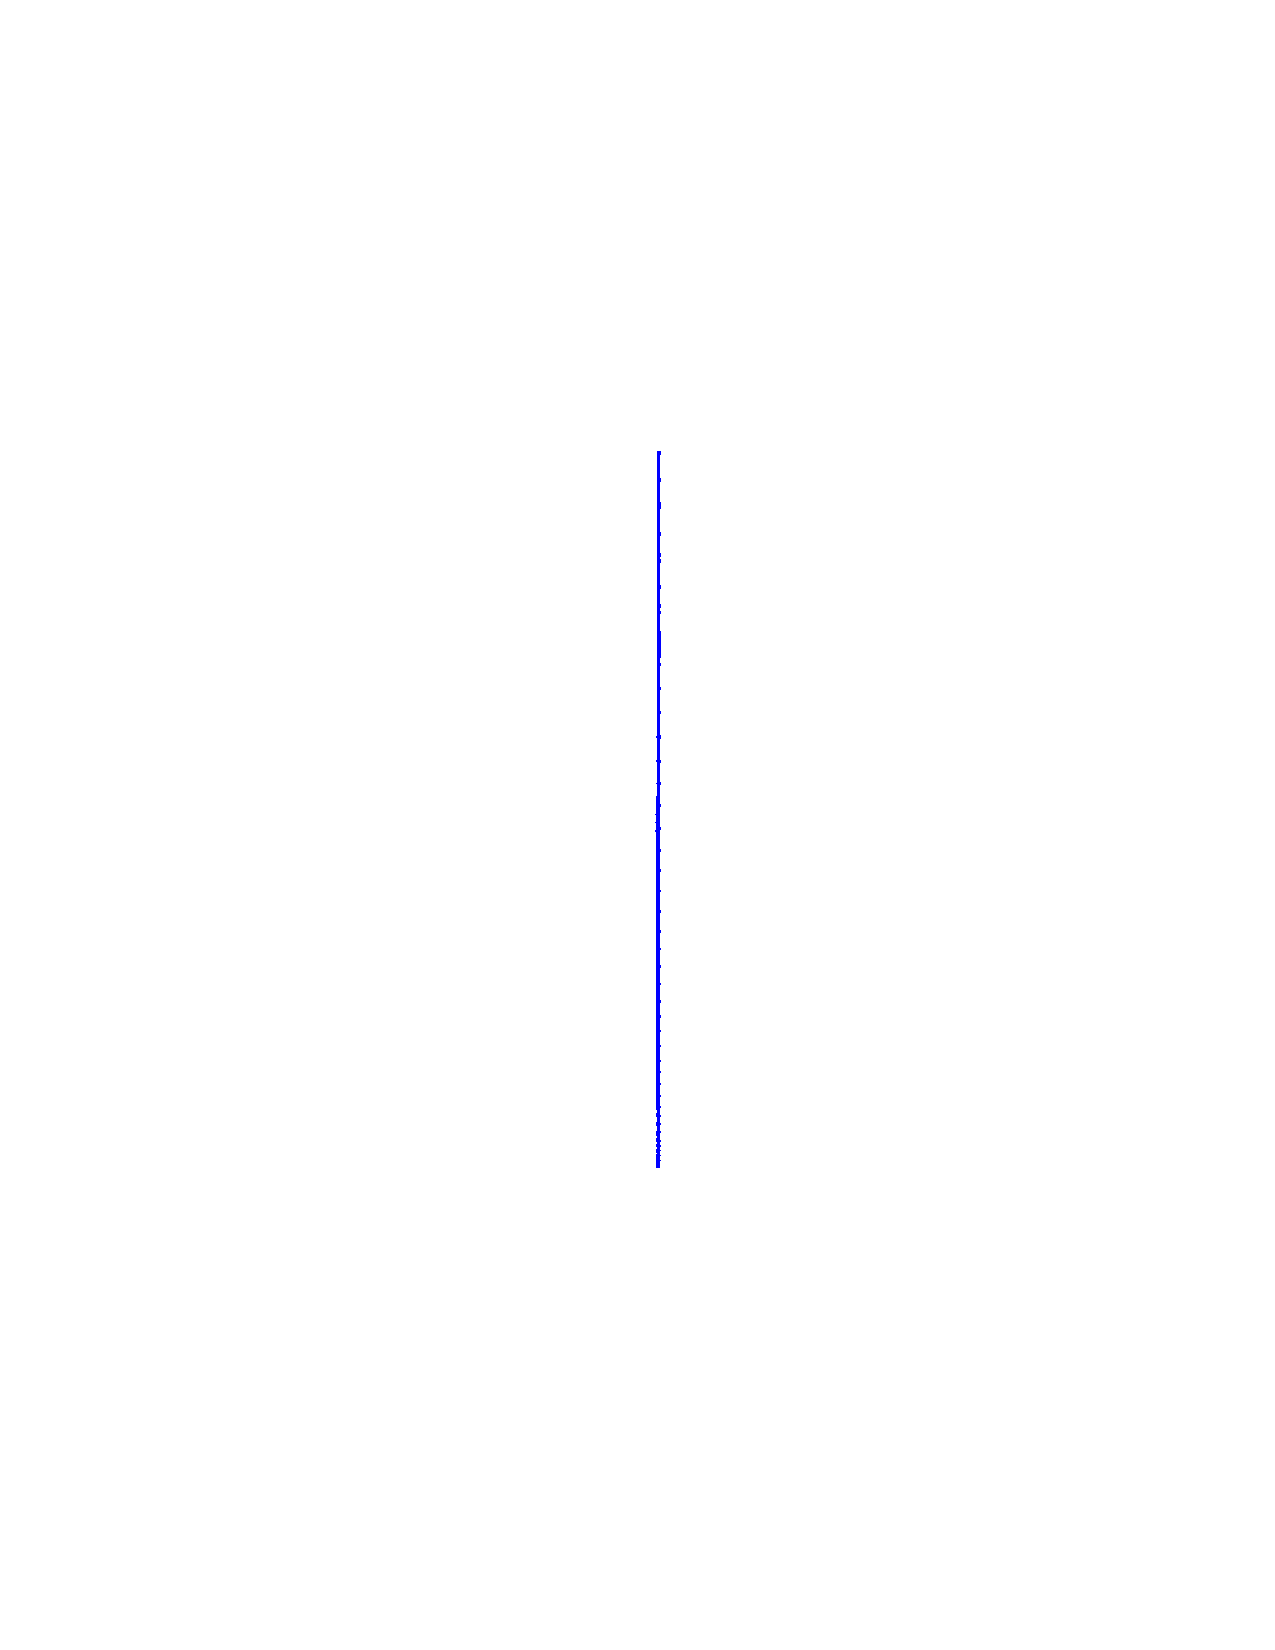
\includegraphics[trim={5cm 5cm 5cm 5cm},
    width=.85\linewidth]{figures/method/straight-trajector}
  \end{minipage}
  \hfill
  \begin{minipage}[t]{0.3\linewidth}
    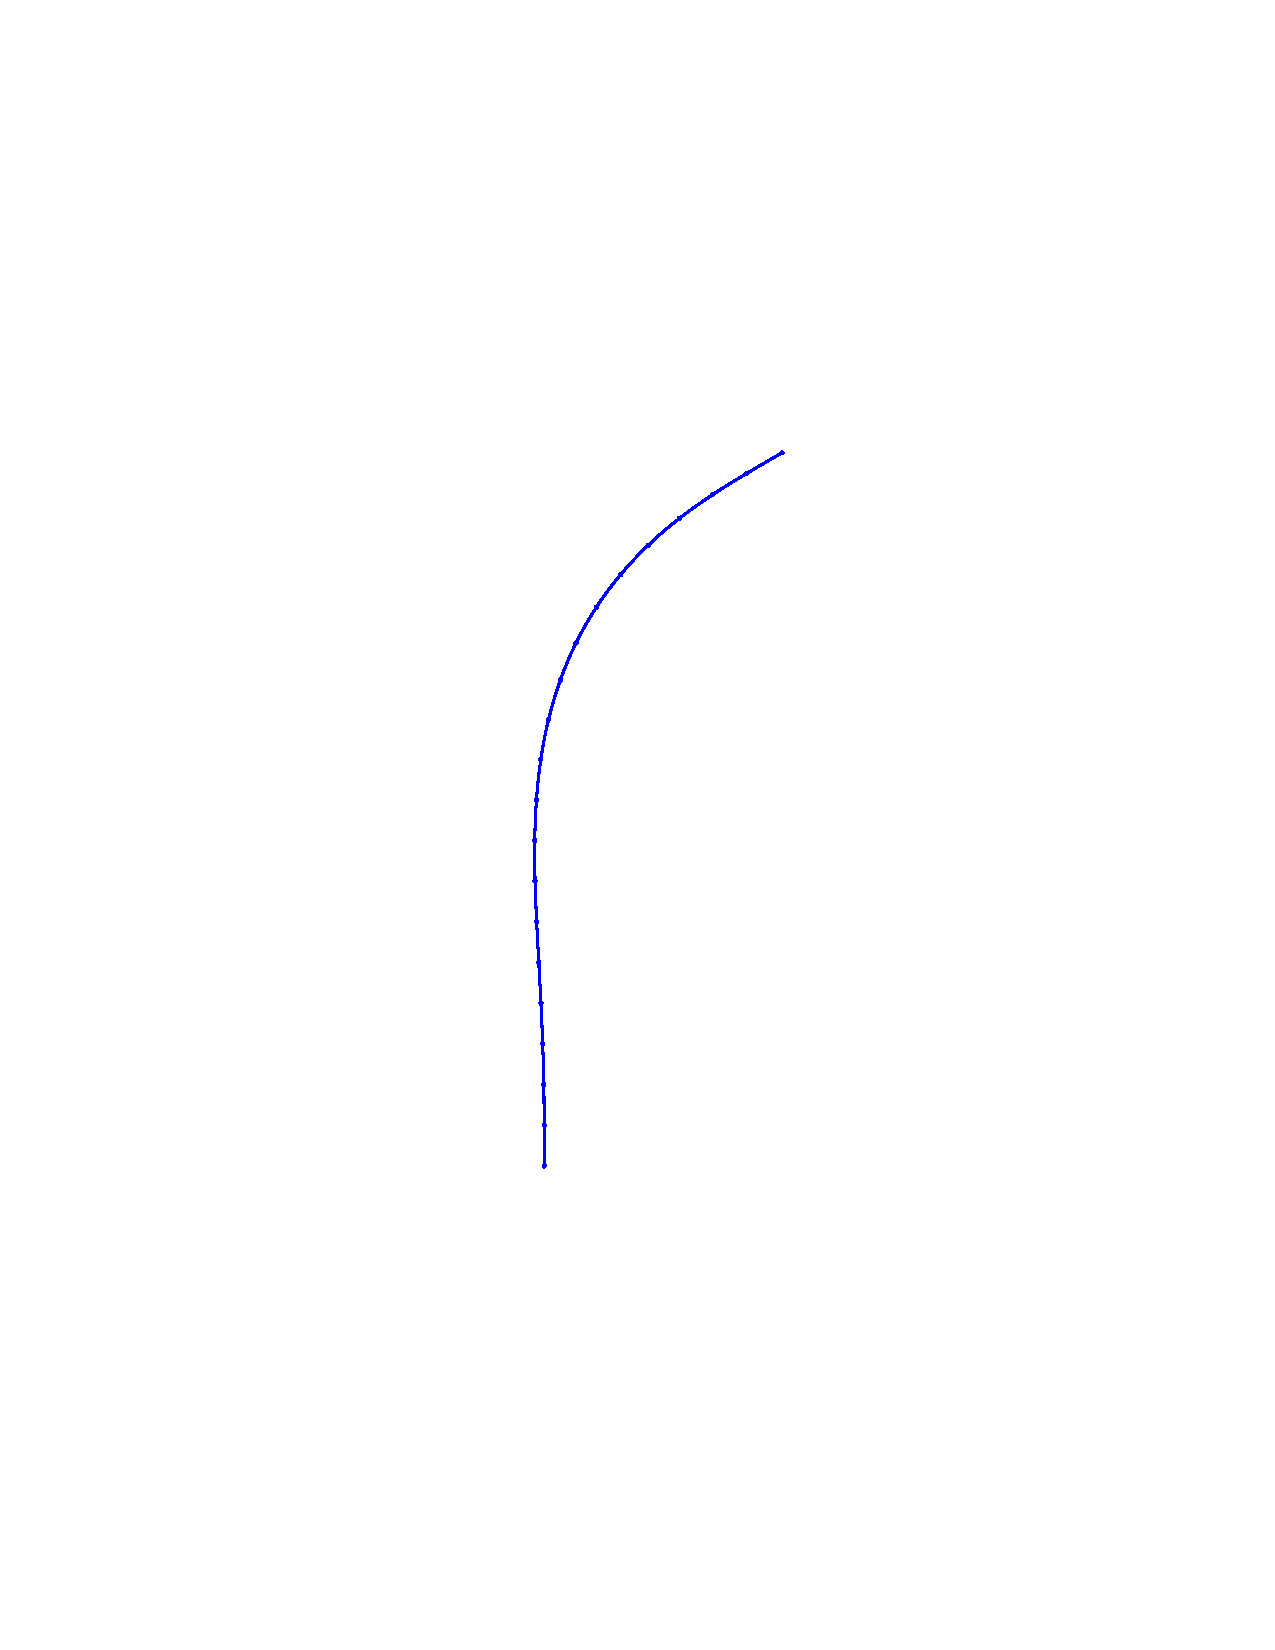
\includegraphics[trim={5cm 5cm 5cm 5cm},
    width=.85\linewidth]{figures/method/right-trajector}
  \end{minipage}
  \caption[Three motion primitives for the \rrtfunnel{} algorithm]{Three motion primitives for the \rrtfunnel{} algorithm, one straight,
    one left, and one right turn.}
  \label{fig:initial-trajectories}
\end{figure}


\subsubsection{Initializing the Funnel Calculations}
\label{subsec:initializing-tvlqr}

The funnel calculation algorithm has to be initialized with a candidate Lyapunov
function. In the same way as in
\citeauthor{majumdarRobustOnlineMotion2013}~\cite{majumdarRobustOnlineMotion2013},
the funnel generation algorithm will be initialized with a \ac{TV-LQR}
controller as the initial Lyapunov function employing a cost function of the
form
\begin{equation}
  J = \vect{x}^{T} (t_f) \matr{F}(t_f) \vect{x} (t_f) + \int_{t_{0}}^{t_{f}} \left( \vect{x}^{T} \matr{Q} \vect{x} + \vect{u}^{T} \matr{R} \vect{u} + 2 \vect{x}^T \matr{N} \vect{u} \right) \mathrm{d}t,
\end{equation}
which when employed on the linearization of the system error
dynamics~\eqref{eq:system-error-dynamics} gives
\begin{equation}
  \dot{\bar{\vect{x}}} \approx \matr{A} (t)\bar{\vect{x}}(t) + \matr{B}(t) \bar{\vect{u}}(t)
\end{equation}
\begin{equation}
  \dot{\bar{\vect{x}}} \approx %
  \begin{bmatrix}
    0 & 0 & -v\cos(\theta) \\
    0 & 0 & -v\sin(\theta) \\
    0 & 0 & 0 \\
  \end{bmatrix} %
  \bar{\vect{x}} (t) %
  + %
  \begin{bmatrix}
    0 \\ 0 \\ 1
  \end{bmatrix} %
  \bar{\vect{u}}(t),
\end{equation} 
which is an an initial candidate Lyapunov function of the form
\begin{equation}
  V(t,\bar{\vect{x}}) = {\bar{\vect{x}}}^{T} \matr{S}_{i}\bar{\vect{x}} ,
\end{equation}
where \(S_{i}\) is a solution of the \textit{Ricatti} equation
\begin{equation}
  \label{eq:ricatti}
  - \dot{\matr{S}}(t) = \matr{A}^{T} \matr{S}(t) +\matr{S}(t) \matr{A} - \left( \matr{S}(t) \matr{B} + \matr{N} \right) \matr{R}^{-1}\left( \matr{B}^{T} \matr{S}(t) + \matr{N}^{T} \right) + \matr{Q}
\end{equation} 
associated with the \ac{LQR} controller. The feedback is gained from
\[
  \matr{K}(t) = \matr{R}^{-1} \left( \matr{B} \matr{S}(t) + \matr{N}^T \right),
\]
and enables the system dynamics \cref{eq:model-dynamics} to be written
\(f_{\mathit{cl}}(t,\vect{x})\) by direct substitution of \(\vect{u} =
-K\vect{x}\), and hence making the system \cref{eq:model-dynamics} only
dependent on \(t\) and \(\vect{x}\),
\begin{equation}
  \label{eq:model-dynamics-cl}
  \vect{x} =
  \begin{bmatrix}
    x \\ y \\ \theta \\
  \end{bmatrix}, \, \dot{\vect{x}} =
  \begin{bmatrix}
    -v \sin(\theta) \\
    v \cos(\theta) \\
    -K\vect{x} \\
  \end{bmatrix} \mathEoS
\end{equation}


\subsection{Generating Funnels Around Trajectories}
\label{subsec:generating-funnels}

With the nominal trajectories, and the initial Lyapunov functions ready, the
funnels around the nominal trajectories can be calculated using
\cref{alg:funnelalgorithm} on page~\pageref{alg:funnelalgorithm}, and is
implemented in software through the \textsc{sostools}~\cite{sostools} toolbox as
shown in \cref{sec:sos-program-implementation}.

However, the dynamics for the model in \cref{eq:model-dynamics-cl} are still not
polynomial, given the \(\sin\) and \(\cos\) terms
in~\eqref{eq:model-dynamics-cl}, and the \ac{SOS}-framework can only verify
polynomial systems. Thus in order to obtain the needed polynomial dynamics, the
system is expanded around the nominal trajectory with a Taylor expansion of
degree three. The function limiting the size of the funnel \(\rho(t_{k})\) also
has to be initialized by a feasible upper bound \(\rho(t)\). This is done
through the equation
\begin{equation}
  \rho(t_{k}) = \mathrm{exp}\left( \rho_{\tau}\frac{\left( t_{f} - t \right)}{\left( t_{f} - t_{0}  \right)}\right) + \rho_0
\end{equation}
where \(\rho_{\tau}\) is a positive constant determining the upper bound on the
funnel, along with the zero value \(\rho_0\)~\cite{Tobenkin_2011}. If the given
choice of \(\rho_{\tau}\) does not verify a funnel, either increase the value of
\(\rho_{\tau}\) and \(\rho_0\), and optionally the number of sampled points from
the trajectory to be verified~\cite{Tobenkin_2011}.

The initial condition set also has to be decided before the reachable set can be
calculated. In general the initial condition set can be any semi-algebraic set
in the state-space. However, a simple way of obtaining an initial condition set
for the trajectories at hand is by taking advantage of the Lyapunov function
candidate from the \ac{LQR}-controller. Thus by setting
\begin{equation}
  \mathcal{X}_{0} = \frac{ \matr{S}_{k}}{\rho_{\tau}},
\end{equation}
an initial condition set is obtained. In general however, any semi-algebraic set
will do, and the algorithm is not constrained to this one initial condition set
in particular, but it has proven itself useful when calculating new motion
primitives for a system when the initial condition set is not obvious. Another
idea is to use the outlet of one funnel as the initial condition set for the
calculation of the next.

The funnels in this thesis are parameterized as sub-level sets of a Lyapunov
function for which the state-space does not invalidate the sub-level constraint.
A visualization of the Lyapunov function associated with a straight motion
primitive can be found in~\cref{fig:visualized-lyapunov}.
\begin{figure}[!t]
  \centering
  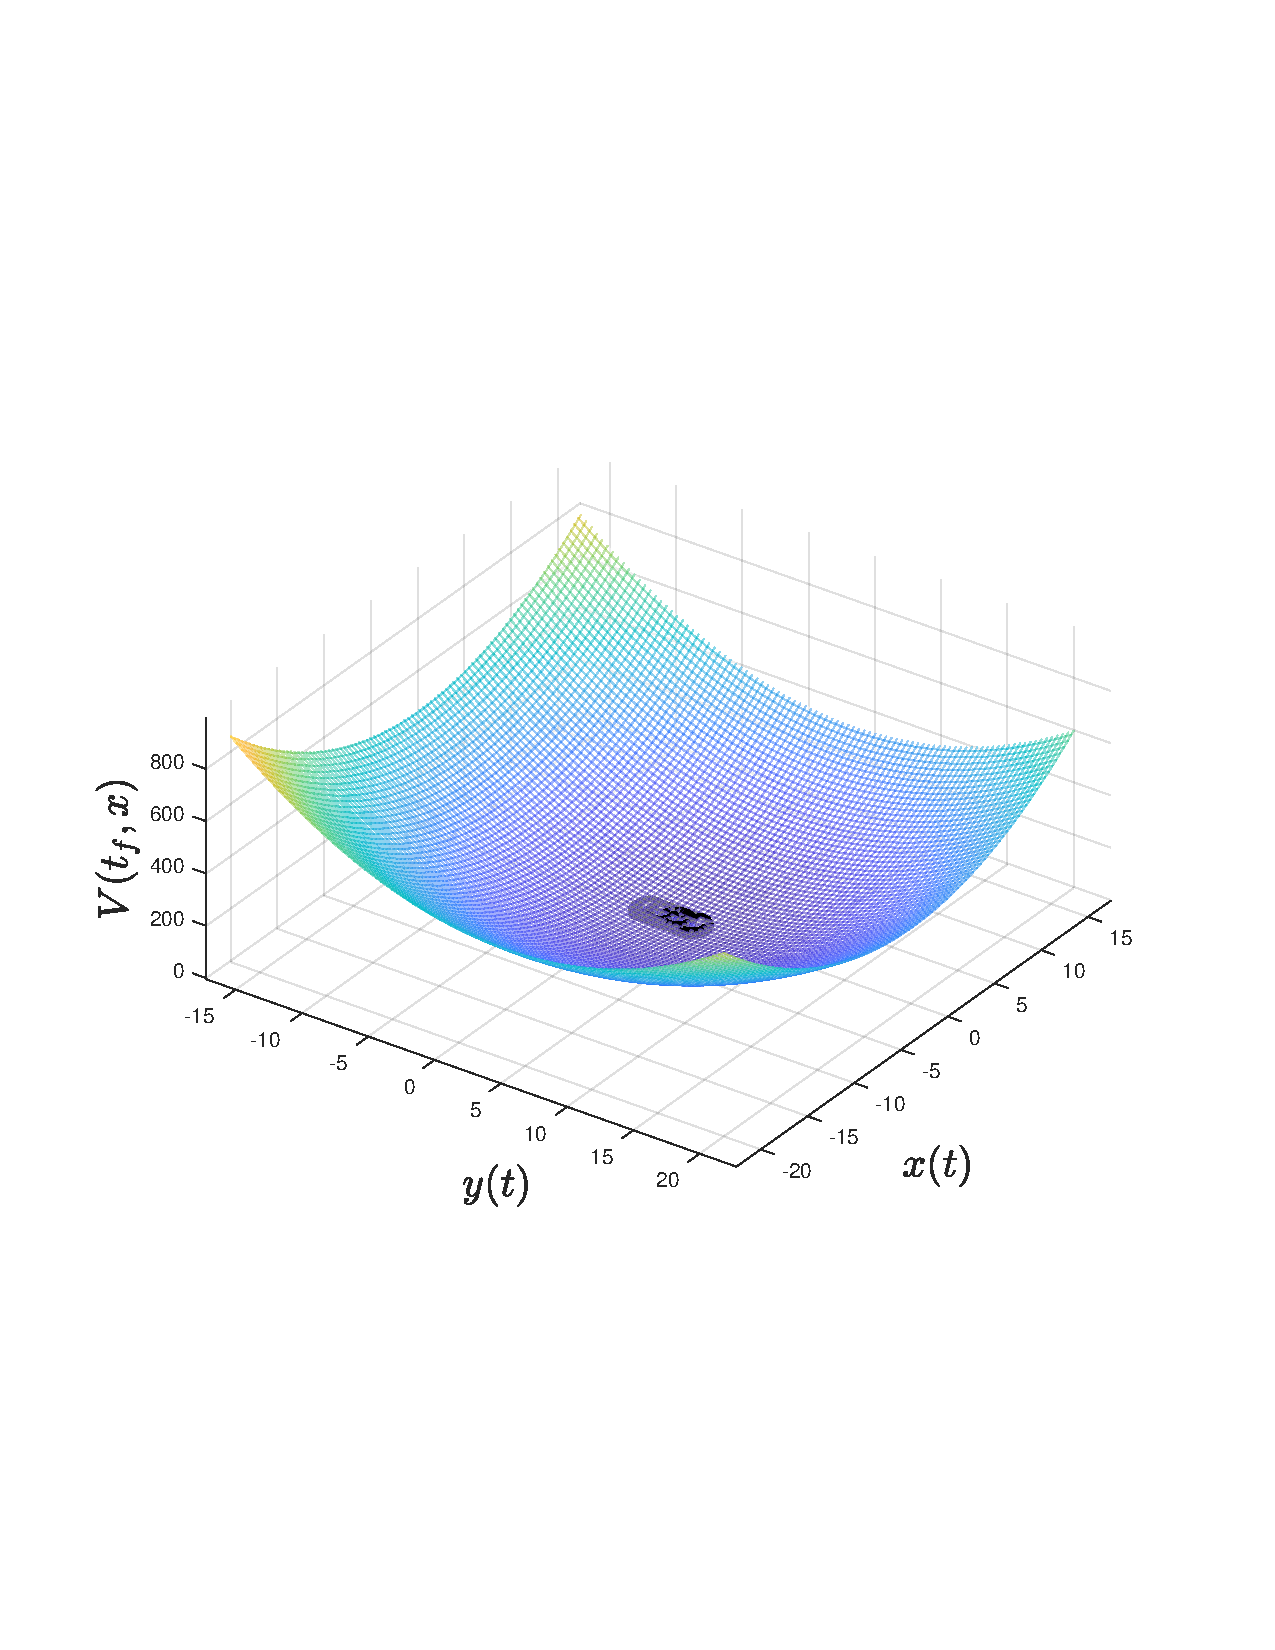
\includegraphics[trim={3cm 7cm 3cm 7cm},
  scale=.6]{figures/rrtfunnel/straight-funnel-lyapunov-3d}
  \caption[The Lyapunov function visualized around a straight trajector]{A visualization of the Lyapunov function values around a straight
    motion primitive.}
  \label{fig:visualized-lyapunov}
\end{figure}

However, for the funnels in this thesis, the initial condition set will be given
by the hyper-ellipsoid
\begin{align}
  \mathcal{X}_0 &= \set{\vect{x} \in \R^{3} \mid \vect{x}^{T} Q \vect{x}} \\
  Q &= \begin{bmatrix}
    2 & 0 & 0 \\
    0 & 2 & 0 \\
    0 & 0 & 4
  \end{bmatrix},
\end{align}
which means that the funnel will have a diameter of one half in the xy-plane,
and the \(\theta\) inlet will be wider closer to the center of the funnel, which
is beneficial, as this is where most of the paths in the experiment setup is
expected to enter.


\subsection{Minimizing the Projected Volume of the Funnel}
\label{subsec:xy-cost-function}

In the \rrtfunnel{} algorithm, the size of the of the hyper-ellipsoid which
contains the reachable set is not equally important in all dimensions for all
planning problems. In the forest traversal case from the introduction, the size
of the ellipsoid in the \(\theta\) dimension is unimportant. There is no need in
minimizing the value of \(\theta\), as it will not make the traversal of the
forest any easier, in fact it might inflate the size of the \((x,y)\) ellipsoid.
As an example: For the dynamical model \eqref{eq:model-dynamics} the size of the
funnel projected down into the xy-plane will be the most important metric.
Whether or not the airplane's orientation parameter \(\theta\) is close to the
nominal heading is of less concern, and is therefore down-prioritized. Having a
large \(\theta\) semi-axis in the hyper-ellipsoid can also be beneficial, as it
increases the inlet of the ellipsoid, which is beneficial if the funnel is to be
composed with another funnel at some other point in the planning process.

For the cost function in the funnel generation \cref{alg:funnelalgorithm} on
page~\pageref{alg:funnelalgorithm}, which in general is a maximization of the
determinant of the upper bound ellipse for the funnel set, it is beneficial to
modify the cost function to penalize the size of the
xy-ellipsoid~\cite{majumdarRobustOnlineMotion2013}.

Therefore in order to minimize the actual size of the funnel where the physical
airplane can move in the world space, the cost function has to be modified. This
can be done through a projection map \(\pi \colon \R^n \rightarrow \R^{n_p}\),
which gives the ellipsoid of interest as \( \mathcal{E} = \set{\bar{\vect{x}}
  \in \R^n \mid \bar{\vect{x}}^TS_{k}\bar{\vect{x}} \leq 1} \mathEoS \) With the
projected ellipsoid given by \( \pi(\mathcal{E}) = \set{\bar{\vect{x}} \in \R^n
  \mid \bar{\vect{x}}^TS^{(p)}_{k}\bar{\vect{x}} \leq 1}, \) where \( S_k^{(p)}
= \p{PS_k^{-1}P^T}^{-1}, \) and \(P\) is an \(n\times n_p\) projection matrix.

Since minimizing the volume of the ellipsoid \(\pi(\mathcal{E})\) using a
\acl{SDP} relies on maximizing the determinant of \(\matr{S}_k\), and \(\deter(
\matr{S}_k)\) is a nonlinear function of \(S_k\), the function has to be
linearized in order for it to be handled by the \ac{SOS} framework.
\citeauthor{majumdarFunnelLibrariesRealtime2017}~\cite{majumdarFunnelLibrariesRealtime2017}
solves this by linearizing \(\deter(\matr{S}_k)\) at the solution of
\(\matr{S}_k\) from the previous iteration, and maximizes this linearization
instead. In the end this translates to
\begin{equation}
  \lin \bigl( \deter \p{ \matr{S}_k} \bigr) = \Tr \bigl( \matr{P}^{T}{\p{ \matr{P}
      \matr{S}_{k,0}^{-1} \matr{P}^T}}^{-1} \matr{P} {\matr{S}_{k,0}}^{-1}
    \matr{S}_k {\matr{S}_{k,0}}^{-1} \bigr),
\end{equation} 
where \( \matr{S}_{k,0}\) is the nominal value for the linearization, and \(\Tr\)
is the trace of the matrix.

\subsection{Optimization of the Nominal \ac{LQR}-Controller}
\label{subsec:searching-for-a-controller}

With the non-optimal feedback controller given to the funnel calculation
framework (non-optimal with regards to the funnel calculation cost function),
the size of the funnels will in general be larger than if the optimizer is given
a better controller. Thus in order to further minimize the size of the funnel in
the xy-plane, this method, along with the cost function from
\cref{subsec:xy-cost-function} is used to make traversal through obstacles in
the world space easier, through minimizing the size of the reachable set. Hence,
the initial controller fed to the algorithm can be optimized with the goal of
minimizing the size of the funnel, given a few conditions on the
system~\cite[sec~4.3.2]{majumdarFunnelLibrariesRealtime2017}.

In order for the controller to be optimized, the system needs to be control
affine\ie it can be written on the form
\begin{equation}
  \dot{\vect{x}} = f(\vect{x}(t)) + g(\vect{x}(t)) \vect{u} (t),
\end{equation}
so that the control policy can be parameterized as a polynomial
\(\bar{\vect{u}}_f(t,\bar{\vect{x}})\), and the system dynamics written as
\begin{equation}
  \label{eq:dynamics-control-affine}
  \dot{\bar{\vect{x}}} = f(\vect{x}_0(t) + \bar{\vect{x}}(t)) + g(\vect{x}(t))\left[ \vect{u}_0(t) + \bar{\vect{u}}_f(t,\bar{\vect{x}}) \right] - \bar{\vect{x}}_0 \mathEoS
\end{equation}
Given that the dynamical model in \cref{eq:model-dynamics} is control affine,
since
\begin{equation}
  \dot{\vect{x}} = %
  f(\vect{x}(t)) + g(\vect{x}(t)) \vect{u} (t) = %
  \begin{bmatrix}
    -v(t)\sin (\theta) \\
    v(t) \cos (\theta) \\
    0
  \end{bmatrix}
  +
  \begin{bmatrix}
    0 \\
    0 \\
    1 \\
  \end{bmatrix}
  \vect{u}(t),
\end{equation}
the feedback controller can be optimized by adding the coefficients of the
polynomial \(\vect{u}_f(t,\bar{\vect{x}})\) to the set of decision variables in
the original optimization problem~\eqref{opt:discrete}. The only issue is
that now \(\dot{V}\) is bilinear in the decision variables \(V\) and
\(\bar{\vect{u}}_f\), as well as the other bilinear decision variables from the
previous formulation, as can be seen from
\begin{equation}
  {
    \newcommand{\Vdot}{\dot{V}}
    \Vdot(t,\vect{x}) = \frac{\partial V(t,\vect{x})}{\partial \vect{x}} \dot{\bar{\vect{x}}} + \frac{\partial V(t,\vect{x})}{\partial t},
  }
\end{equation}
where \(\dot{\bar{\vect{x}}}\) is now given by
\cref{eq:dynamics-control-affine}. Thus in order to optimize the control input a
search is done in the variables \( (\bar{\vect{u}}_f,\rho,L_t,L_{0,i},S_k) \)
while keeping \( (V,L,L_{\epsilon,k}) \) fixed. This method combined with the
uncertainty added in~\cref{sec:adding-uncertainty}, is what forms the basis for
the funnel computations as robust motion primitives for traversal in a dense
forest environment, as summarized in \cref{alg:funnelalgorithm-extended}
(Optimization 2).

\begin{algorithm}[H]
  \caption{Feedback Funnel computation} \label{alg:funnelalgorithm-extended}
  \begin{algorithmic}[0]
    \Procedure{Feedback Funnel Computation}{$a,b$}\Comment{Computes the feedback funnel}
    \State \(cost_{prev} = \infty\)
    \State converged = false
    \While{\( \neg converged\)}
    \State Optimization problem 1:
    \State %
    \begin{align*}
      \underset{\substack{\bar{u}_f,L,L_{t},L_{0,i},S_{k},L_{}}}{\inf}&  \sum_{k=1}^{N} \vol \bigl( \mathcal{E}(t_{k}) \bigr) & \\    
      \text{subject to } & V \text{ and } \rho \text{ constant.}& \\
    \end{align*}
    \State Optimization problem 2:
    \State %
    \begin{align*}
      \underset{\substack{\bar{u}}_f,\rho,L_{t},L_{0,i},S_{k}}{\inf}&  \sum_{k=1}^{N} \vol \bigl( \mathcal{E}(t_{k}) \bigr) & \\    
      \text{subject to } & (V,L,L_{\mathcal{E},k}) \text{ constant.}& \\
    \end{align*}
    \State Optimization problem 3:
    \State %
    \begin{align*}
      \underset{\substack{V,\rho, L_{t},L_{0,i},S_{k}}}{\inf}&  \sum_{k=1}^{N} \vol \bigl( \mathcal{E}(t_{k}) \bigr) & \\    
      \text{subject to } & (L,L_{\mathcal{E},k},\bar{u}_f) \text{ constant.}& \\
    \end{align*}
    \State cost = \(\sum_{k=1}^{N} \vol \bigl( \mathcal{E}(t_{k}) \bigr) \)
    \If{\(\frac{cost_{prev} - cost}{cost_{prev}} < \epsilon\)}
    \State converged = true
    \EndIf
    \State \(cost_{prev} = cost\)
    \EndWhile
    \EndProcedure
  \end{algorithmic}
\end{algorithm}
